% \chapter{Theoretical Background}\label{chap:theoretical background}

% \section{Example citation \& symbol reference}\label{sec:citation}
% For symbols look at \cite{latex_symbols_2017}.


% \section{Example reference}
% Example reference: Look at chapter~\ref{chap:introduction}, for sections, look at section~\ref{sec:citation}.

% \section{Example image}

% \begin{figure}
% 	\centering
% 	\includegraphics[width=0.5\linewidth]{uni-logo}
% 	\caption{Meaningful caption for this image}
% 	\label{fig:uniLogo}
% \end{figure}

% Example figure reference: Look at Figure~\ref{fig:uniLogo} to see an image. It can be \texttt{jpg}, \texttt{png}, or best: \texttt{pdf} (if vector graphic).

% \section{Example table}

% \begin{table}
% 	\centering
% 	\begin{tabular}{lr}
% 		First column & Number column \\
% 		\hline
% 		Accuracy & 0.532 \\
% 		F1 score & 0.87
% 	\end{tabular}
% 	\caption{Meaningful caption for this table}
% 	\label{tab:result}
% \end{table}

% Table~\ref{tab:result} shows a simple table\footnote{Check \url{https://en.wikibooks.org/wiki/LaTeX/Tables} on syntax}

\chapter{Background on learning on graphs}\label{chap:background}
The following sections provide an overview of the concepts and methods related to graph theory, machine learning, and graph neural networks. 

\section{Notion}
At first, we need to define some terms with regard to the graph. In graph theory, we assume that $G=(V,E)$ is an undirected graph, where $V$ is the set of nodes and $E  \subseteq \{\{v,w\}\mid v,w \in V , v \neq w\}$ is the set of edges. We use $\mathbb{G}$ to represent the set of all possible graphs. The neighborhood of a node $v$ is denoted as $N(v)$, defined as $N(v) = \{w \mid \{v,w\} \in E\}$. The degree of a node $v$, denoted as $d(v)$, is the number of neighbors of $v$, that is, $d(v) = |N(v)|$. In addition to the nodes and edges that comprise the graph, we can attach a more complex set of data to each node.  A feature vector $x_n\in \mathbb{R}^k$, is attached to a node $v_n$, and in some cases, edge feature vectors are also included. These vectors can be used to characterize graphs or nodes in graphs. The adjacency matrix $A \in \mathbb{R}^{|V| \times |V|}$ is a matrix that represents the connections between nodes in the graph. The element $a_{ij}$ of the adjacency matrix is 1 if there is an edge between node $v_i$ and node $v_j$, and 0 otherwise.

\section{Machine learning}
In the following section, we provide an overview of the concepts and methods related to machine learning. 

\paragraph{Supervised learning}
Machine learning can be roughly divided into three categories: supervised learning, unsupervised learning, and reinforcement learning~\cite{bishop2006pattern}.

Supervised learning is a type of machine learning that involves training a model on a labeled dataset. The model is trained to learn the relationship between the input features and the output labels. The goal is to learn a mapping from the input features to the output labels so that the model can make predictions on new, unseen data. One common task in supervised learning is classification, where the goal is to assign each input vector to one of a finite number of classes (categories). In the graph learning context, the predicted output can be a label for each node in the graph, a label for the entire graph, or a label for each edge in the graph, e.g. node classification, graph classification, and link prediction~\cite{velivckovic2023everything}.

\paragraph{Feed-forward neural networks}

Feed-forward neural networks, also known as multilayer perceptrons (MLPs), are a type of neural network that consists of multiple layers of neurons. The neurons in each layer are connected to the neurons in the next layer, and the output of each neuron is computed as a weighted sum of the inputs followed by a non-linear activation function. The output of the network is computed by passing the input through the network and computing the output of the final layer. The weights of the network are learned by using an optimization algorithm such as gradient descent. Feed-forward neural networks are a powerful tool for learning complex patterns in data and have been successfully applied to a wide range of tasks, such as image recognition, speech recognition, and natural language processing.

The function of a feed-forward neural network can be written as

$$ 
    y = f(W^{(L)} \cdot f(W^{(L-1)} \cdot \ldots \cdot f(W^{(1)} \cdot x + b^{(1)}) + b^{(2)}) + \ldots + b^{(L)})
$$

where $x$ is the input vector, $W^{(i)}$ and $b^{(i)}$ are the weights and biases of the $i$-th layer, and $f$ is the activation function. The output $y$ is the predicted output of the network. $L$ is denoted as the depth of the network. See Figure~\ref{fig:neural_network} for an illustration of a single neuron in a feed-forward neural network.

\usetikzlibrary{decorations.pathreplacing}
\begin{figure}[h!]
    \centering
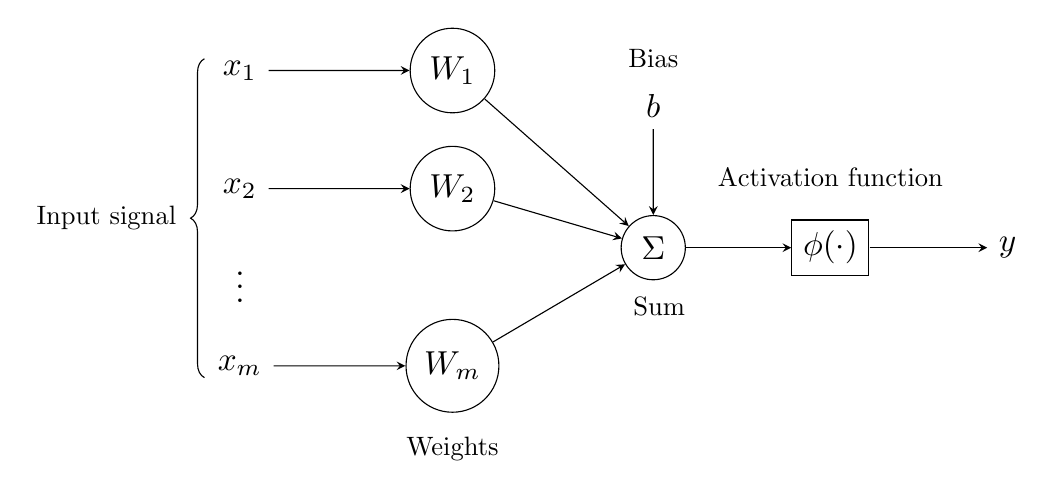
\begin{tikzpicture}[>=stealth, scale=1.5, every node/.style={scale=1.2}]

    % Input signals
    \node at (-1.5, 1.5) (x1) {$x_1$};
    \node at (-1.5, 0.5) (x2) {$x_2$};
    \node at (-1.5, -1) (xm) {$x_m$};
    \node at (-1.5, -0.25) (dots) {$\vdots$};
    
    % Input brackets
    \draw[decorate, decoration={brace, amplitude=5pt}] (-1.8, -1.1) -- (-1.8, 1.6) node[midway, left, xshift=-0.2cm, scale=0.8] {Input signal};
        
    % Weights
    \node[draw, circle] at (0.3, 1.5) (w1) {$W_1$};
    \node[draw, circle] at (0.3, 0.5) (w2) {$W_2$};
    \node[draw, circle] at (0.3, -1) (wm) {$W_m$};
    
    \draw[->] (x1) -- (w1);
    \draw[->] (x2) -- (w2);
    \draw[->] (xm) -- (wm);

    % Sum node
    \node[draw, circle] at (2, 0) (sum) {$\Sigma$};
    
    % Weighted connections to sum
    \draw[->] (w1) -- (sum);
    \draw[->] (w2) -- (sum);
    \draw[->] (wm) -- (sum);
    
    % Bias
    \node[scale=0.8] at (2, 1.6) (biasText) {Bias};
    \node at (2, 1.2) (biasEq) {$b$};
    \draw[->] (biasEq) -- (sum);
    
    % Activation function
    \node[draw, rectangle] at (3.5, 0) (activation) {$\phi(\cdot)$};
    \node at (5, 0) (y) {$y$};
    \draw[->] (sum) -- (activation);
    \draw[->] (activation) -- (y);
    
    % Activation function label
    \node[scale=0.8] at (3.5, 0.6) {Activation function};
    
    % Weight label
    \node[scale=0.8] at (0.3, -1.7) {Weights};
    
    % Sum label
    \node[scale=0.8] at (2.05, -0.5) {Sum};
\end{tikzpicture}
\caption{An illustration of a single neuron in a feed-forward neural network. The neuron computes a weighted sum of the input signals, adds a bias term, and applies an activation function to produce the output.}
\label{fig:neural_network}
\end{figure}

\paragraph{Loss function}
The loss function is a function that measures the difference between the predicted output of a model and the true output. The goal of training a machine learning model is to minimize the loss function, which is done by adjusting the parameters of the model using an optimization algorithm such as gradient descent. The choice of loss function depends on the task at hand. For classification tasks, the cross-entropy loss function is commonly used, while for regression tasks, the mean squared error loss function is often used.

The cross-entropy loss function is defined as 

$$
    L(y, \hat{y}) = -\sum_{i} y_i \log(\hat{y}_i)
$$

where $y$ is the true output, $\hat{y}$ is the predicted output, and $i$ is the index of the classes. The cross-entropy loss function is used to measure the difference between the true output and the predicted output of a classification model. See Figure~\ref{fig:loss_function} for an example of a cost function surface in machine learning.

\begin{figure}[H]
    \centering
    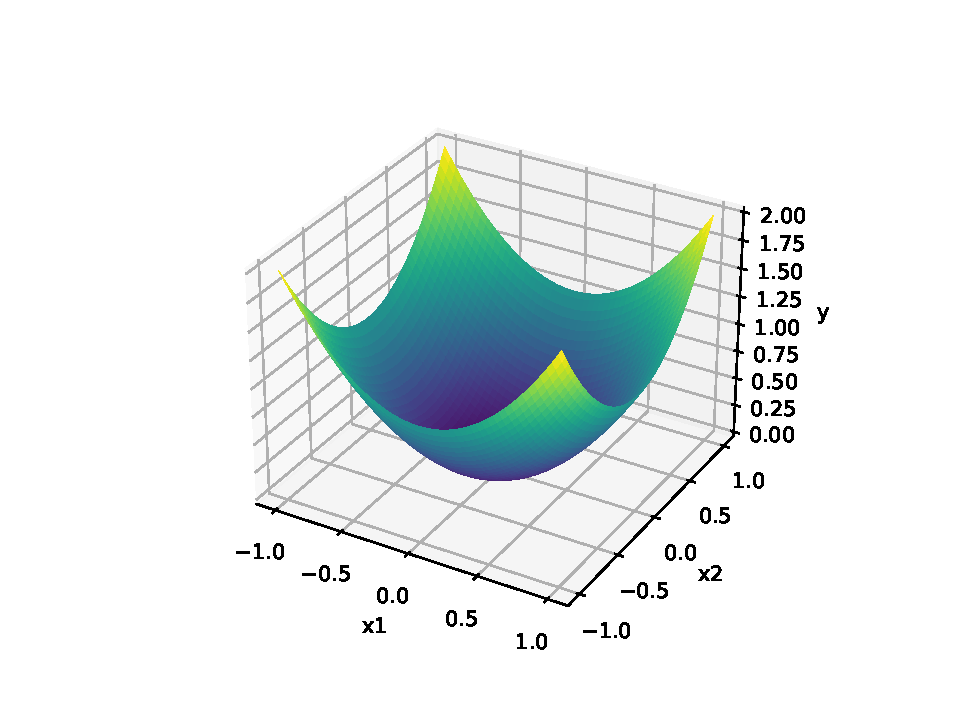
\includegraphics[width=0.8\textwidth]{loss_function.pdf}
    \caption{3D representation of a cost function surface in machine learning. Optimization algorithms aim to navigate this surface to reach the global minimum, improving model accuracy.}
    \label{fig:loss_function}
\end{figure}

\paragraph{Activation function}
An activation function is a non-linear function that is applied to the output of a neuron in a neural network. The activation function introduces non-linearity into the network, allowing it to learn complex patterns in the data. There are many activation functions that can be used in neural networks, such as the sigmoid function, the tanh function, and the ReLU function. The ReLU function is one of the most commonly used activation functions in deep learning because it is simple and computationally efficient. The ReLU function is defined as

$$
    \textrm{ReLU}(\cdot)=\max(0,\cdot)
$$

The ReLU function is used to introduce non-linearity into the network and has been shown to be effective in training deep neural networks.


\paragraph{Gradient Descent}
Gradient descent is an optimization algorithm used to minimize a function by iteratively moving in the direction of the steepest decrease of the function. The algorithm works by computing the gradient of the function at a given point and then updating the point in the direction of the negative gradient. The update rule is given by

$$
    W^{(t+1)} = W^{(t)} - \alpha \nabla f(W^{(t)})
$$
where $W^{(t)}$ is the parameter vector at iteration $t$, $\alpha$ is the learning rate, and $\nabla f(W^{(t)})$ is the gradient of the function $f$ with respect to the parameters $W^{(t)}$. The learning rate $\alpha$ is a hyperparameter that controls the step size of the update. Gradient descent is a popular optimization algorithm used in machine learning to train neural networks and other models.

\paragraph{Stochastic Gradient Descent}
Stochastic gradient descent (SGD) is a variant of gradient descent that uses a random sample of the training data to compute the gradient at each iteration. The algorithm works by randomly selecting a mini-batch of data points from the training dataset, computing the gradient of the loss function with respect to the mini-batch, and then updating the parameters based on the gradient. The update rule is given by

$$
    W^{(t+1)} = W^{(t)} - \alpha \nabla f(W^{(t)}, x^{(t)})
$$
where $x^{(t)}$ is a mini-batch of data points from the training dataset. Stochastic gradient descent is more computationally efficient than standard gradient descent and can be used to train large-scale machine learning models.

\paragraph{Early Stopping}
Early stopping is a technique used to prevent overfitting in machine learning models. The idea is to monitor the performance of the model on a validation dataset during training and stop training when the performance starts to degrade. This is done by keeping track of the validation loss and stopping training when the validation loss stops decreasing or starts to increase. Early stopping is used to prevent the model from memorizing the training data and to obtain a more generalizable model. 

\paragraph{Cross-validation}
Cross-validation is a technique used to evaluate the performance of a machine learning model. The idea is to split the dataset into multiple subsets, or folds, and train the model on one subset while evaluating it on the remaining subsets. This process is repeated multiple times, with each subset used as the test set once. The performance of the model is then averaged over all the folds to obtain an estimate of the model's generalization performance. Cross-validation is used to prevent overfitting and to obtain a more accurate estimate of the model's performance. See Figure~\ref{fig:cross-validation} for an example of 5-fold cross-validation.


\begin{center}
    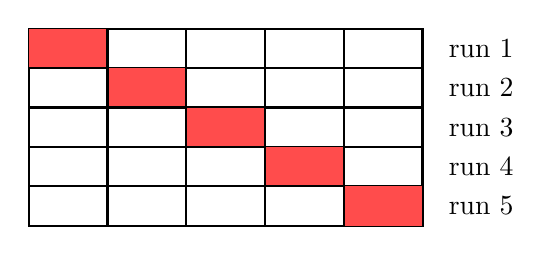
\begin{tikzpicture}[scale=1.0]

    % Run 1
    \draw[thick] (0, 5) rectangle (5, 5.5);
    \fill[red!70] (0, 5) rectangle (1, 5.5);
    \draw[thick] (1, 5) -- (1, 5.5);
    \draw[thick] (2, 5) -- (2, 5.5);
    \draw[thick] (3, 5) -- (3, 5.5);
    \draw[thick] (4, 5) -- (4, 5.5);

    \node[right=6pt] at (5, 5.25) {run 1};

    % Run 2
    \draw[thick] (0, 4.5) rectangle (5, 5);
    \fill[red!70] (1, 4.5) rectangle (2, 5);
    \draw[thick] (1, 4.5) -- (1, 5);
    \draw[thick] (2, 4.5) -- (2, 5);
    \draw[thick] (3, 4.5) -- (3, 5);
    \draw[thick] (4, 4.5) -- (4, 5);

    \node[right=6pt] at (5, 4.75) {run 2};

    % Run 3
    \draw[thick] (0, 4) rectangle (5, 4.5);
    \fill[red!70] (2, 4) rectangle (3, 4.5);
    \draw[thick] (1, 4) -- (1, 4.5);
    \draw[thick] (2, 4) -- (2, 4.5);
    \draw[thick] (3, 4) -- (3, 4.5);
    \draw[thick] (4, 4) -- (4, 4.5);
    \node[right=6pt] at (5, 4.25) {run 3};

    % Run 4
    \draw[thick] (0, 3.5) rectangle (5, 4);
    \fill[red!70] (3, 3.5) rectangle (4, 4);
    \draw[thick] (1, 3.5) -- (1, 4);
    \draw[thick] (2, 3.5) -- (2, 4);
    \draw[thick] (3, 3.5) -- (3, 4);
    \draw[thick] (4, 3.5) -- (4, 4);
    \node[right=6pt] at (5, 3.75) {run 4};

    % Run 5
    \draw[thick] (0, 3) rectangle (5, 3.5);
    \fill[red!70] (4, 3) rectangle (5, 3.5);
    \draw[thick] (1, 3) -- (1, 3.5);
    \draw[thick] (2, 3) -- (2, 3.5);
    \draw[thick] (3, 3) -- (3, 3.5);
    \draw[thick] (4, 3) -- (4, 3.5);
    \node[right=6pt] at (5, 3.25) {run 5};

    \end{tikzpicture}
    \captionof{figure}{Example of 5-fold cross-validation, where the dataset is split into 5 folds and the model is trained and evaluated on each fold. The red portion of each fold represents the test set, while the white portion represents the training set. The performance of the model is averaged over all the folds to obtain an estimate of the model's generalization performance.}
    \label{fig:cross-validation}
\end{center}

\paragraph{Hyperparameter tuning}
Hyperparameter tuning is the process of selecting the optimal hyperparameters for a machine learning model. Hyperparameters are parameters that are set before the training process begins and control the behavior of the model. Examples of hyperparameters include the learning rate, batch size, number of hidden layers, and number of epochs. Hyperparameter tuning is an important step in the machine learning pipeline and can have a significant impact on the performance of the model. There are many techniques for hyperparameter tuning, such as grid search, random search, and Bayesian optimization. In this thesis, Bayesian optimization is used to tune the hyperparameters of the models.

Bayesian optimization is more efficient than grid search and random search because it uses a probabilistic model to guide the search for the optimal hyperparameters. The idea is to model the objective function (e.g. the validation accuracy of the model) as a Gaussian process and use the model to select the next set of hyperparameters to evaluate. This process is repeated until the optimal hyperparameters are found.

\paragraph{Optimization algorithm}
An optimization algorithm is an algorithm used to minimize a function by iteratively updating the parameters of the model. The goal is to find the set of parameters that minimizes the loss function. Gradient descent is a common optimization algorithm used in machine learning, but there are many variants of gradient descent that are designed to improve convergence speed and stability. Some popular optimization algorithms include Adam~\cite{kingma2014adam}, RMSprop~\cite{graves2013generating}, and Adagrad~\cite{duchi2011adaptive}. These algorithms use different strategies to update the parameters of the model and can be more effective than standard gradient descent in certain situations. 

\paragraph{Generalization}
A key concept in evaluating model performance or generalization ability in such task is the empirical generalization error $E_{gen}$. This is a measure of how well the model generalizes to unseen data, which can be calculated as the difference between the training accuracy and the test accuracy. It is defined as

$$
    E_{gen} = {Acc_{train}} - {Acc_{test}}
$$
where $Acc_{train}$ is the accuracy of the model on the training dataset, and $Acc_{test}$ is the accuracy of the model on the test dataset. The accuracy $Acc$ on a dataset is defined as the proportion of correctly classified graphs, that is, $Acc = \frac{\textrm{Number of correctly classified graphs}}{\textrm{Total number of data points}}$.

The empirical generalization error is also known as the generalization gap~\cite{goodfellow2016deep}. Typically, the learning on the training dataset and test dataset behaves differently. The model may perform well on the training dataset but poorly on the test dataset. By observing the generalization error, we can decide on a stopping criterion for the training process. And the generalization error can be used to determine whether the model is overfitting or underfitting. Furthermore, the generalization error can be influenced by many factors, such as the model architecture, the hyperparameters, and the data properties in the dataset (e.g. Graph parameter). 

\section{Graph Neural Networks}
Graph Neural Networks (GNNs) are a class of neural networks that can operate on graph-structured data. GNNs use the structure of a graph to perform "message passing", allowing information to propagate across nodes and edges. The key idea is to iteratively aggregate and update node features by exchanging information with local neighboring nodes, which allows GNNs to capture the structural information of the graph. This information is then used to make predictions. GNNs have been demonstrated to be effective in a wide range of tasks, such as node classification, edge prediction, and graph classification. Popular GNNs in recent years include Graph Convolutional Networks (GCN), Graph Attention Networks (GAT), and Message Passing Neural Networks (MPNN).

In the following sections, we provide an overview of the methods related to this thesis.

\paragraph{Graph Convolutional Networks (GCN)}

Graph Convolutional Networks (GCNs) are a class of neural networks that can operate on graph-structured data. The GCN model $f(X, A)$, as proposed by Kipf and Welling~\cite{kipf2016semi}, is defined as

$$ 
 H^{(l+1)} = \sigma(\tilde{D}^{-\frac{1}{2}}\tilde{A}\tilde{D}^{-\frac{1}{2}}H^{(l)}W^{(l)})
$$

where $H^{(l)}\in \mathbb{R}^{N\times D}$ is the node feature matrix at layer $l$; $H^{(0)} = X$. $\tilde{A} = A + I$ is the adjacency matrix of the graph with self-connections added, $\tilde{D}$ is the degree matrix of $\tilde{A}$, $W^{(l)}$ is the weight matrix of the layer, and $\sigma$ is the activation function, such as the $\textrm{ReLU}(\cdot)=\max(0,\cdot)$. The GCN layer aggregates information from neighboring nodes and updates the node features by applying a linear transformation followed by a non-linear activation function. The output of the GCN layer is the node feature matrix at the next layer. The GCN layer can be stacked to create deep GCN models, which have been shown to be effective in a wide range of tasks, such as node classification, edge prediction, and graph classification.


\paragraph{Simplified Graph Convolution (SGC)}

Simplified Graph Convolution (SGC)~\cite{wu2019simplifying} is a simplified version of the GCN model that removes the non-linear activation function and the normalization of the adjacency matrix. The SGC model is defined as

$$
 X' = (\tilde{D}^{-\frac{1}{2}}\tilde{A}\tilde{D}^{-\frac{1}{2}})^K XW
$$

where $X$ is the node feature matrix, $W$ is the weight matrix, $\tilde{A}$ is the adjacency matrix with self-connections added, $\tilde{D}$ is the degree matrix of $\tilde{A}$, and $K$ is the number of layers. 


\paragraph{Graph Attention Networks (GAT)}
Graph Attention Networks (GAT) are a class of neural networks that use attention mechanisms to aggregate information from neighboring nodes. The GAT model updates the feature representation of a node by assigning different importance scores, known as attention coefficients, to its neighbors. The updated node feature $\mathbf{h}_i^{(l+1)}$ at layer $l+1$ is given by:

$$
\mathbf{h}_i^{(l+1)} = \sigma \left( \sum_{j \in \mathcal{N}(i)} \alpha_{ij}^{(l)} \mathbf{W}^{(l)} \mathbf{h}_j^{(l)} \right)
$$

where $\mathbf{h}_i^{(l)}$ is the feature vector of node $i$ at layer $l$, $\mathbf{W}^{(l)}$ is a learnable weight matrix, $\sigma$ is an activation function, and $\alpha_{ij}^{(l)}$ is the attention coefficient between nodes $i$ and $j$. These coefficients are computed as:

$$
\alpha_{ij}^{(l)} = \frac{\exp \left( \textrm{LeakyReLU} \left( \mathbf{a}^{(l)^\top} [\mathbf{W}^{(l)} \mathbf{h}_i^{(l)} \| \mathbf{W}^{(l)} \mathbf{h}_j^{(l)}] \right) \right)}{\sum_{k \in \mathcal{N}(i)} \exp \left( \textrm{LeakyReLU} \left( \mathbf{a}^{(l)^\top} [\mathbf{W}^{(l)} \mathbf{h}_i^{(l)} \| \mathbf{W}^{(l)} \mathbf{h}_k^{(l)}] \right) \right)}
$$

where $\|$ denotes the concatenation of node features, and $\mathbf{a}^{(l)}$ is a shared attention vector. The softmax function ensures the attention coefficients sum to one for a node's neighbors.

GAT is particularly effective for tasks where different neighbors contribute unequally to a node's representation. By using attention mechanisms, GAT dynamically weighs neighbor contributions, enabling more expressive feature aggregation compared to earlier methods like GCNs.

\paragraph{Graph Attention Networks v2 (GATv2)}
Graph Attention Networks v2 (GATv2)~\cite{brody2021attentive} is an improved version of the GAT model that introduces residual connections and multi-head attention. The GATv2 model is defined as

$$
    \mathbf{h}_i^{(l+1)} = \sigma \left( \sum_{h=1}^{H} \sum_{j \in \mathcal{N}(i)} \alpha_{ij}^{(l,h)} \mathbf{W}^{(l,h)} \mathbf{h}_j^{(l)} \right) + \mathbf{h}_i^{(l)}
$$

where $H$ is the number of attention heads, $\alpha_{ij}^{(l,h)}$ is the attention coefficient between nodes $i$ and $j$ for head $h$, and $\mathbf{W}^{(l,h)}$ is the weight matrix for head $h$. The attention coefficients are computed as

$$
    \alpha_{ij}^{(l,h)} = \frac{\exp \left( \textrm{LeakyReLU} \left( \mathbf{a}^{(l,h)^\top} [\mathbf{W}^{(l,h)} \mathbf{h}_i^{(l)} \| \mathbf{W}^{(l,h)} \mathbf{h}_j^{(l)}] \right) \right)}{\sum_{k \in \mathcal{N}(i)} \exp \left( \textrm{LeakyReLU} \left( \mathbf{a}^{(l,h)^\top} [\mathbf{W}^{(l,h)} \mathbf{h}_i^{(l)} \| \mathbf{W}^{(l,h)} \mathbf{h}_k^{(l)}] \right) \right)}
$$

The GATv2 model uses multi-head attention to allow the model to attend to different parts of the input space. The model also introduces residual connections to improve the flow of information through the network. The GATv2 model has been shown to outperform the original GAT model on a wide range of tasks.

\paragraph{Message Passing Neural Networks (MPNN)}
Message Passing Neural Networks (MPNNs)~\cite{gilmer2017neural} have been the leading model for graph learning. The MPNN model operates by iteratively passing messages between nodes and updating their representations. At each iteration $t$, the message vector $m_i^{(t+1)}$ for node $i$ is computed as:

$$
    m_i^{(t+1)} = \sum_{j\in N(i)}M^{(t)}(h_i^{(t)}, h_j^{(t)}, e_{ij})
$$

where $m_i^{(t)}$ is the message vector of node $i$ at iteration $t$, $M^{(t)}$ is a learnable message function (typically implemented as a neural network, such as an MLP), $h_i^{(t)}$ is the node feature vector of node $i$ at iteration $t$, $h_j^{(t)}$ is the node feature vector of node $j$ at iteration $t$, $e_{ij}$ is the edge feature vector between node $i$ and node $j$, and $N(i)$ is the neighborhood of node $i$. The message function $M^{(t)}$ is a neural network that takes as input the node feature vectors of node $i$ and node $j$, and the edge feature vector between them, and outputs the message vector $m_i^{(t)}$.

\section{Graph parameters} \label{sec:graph_parameters}
Now we can introduce the concept of a graph parameter. A graph parameter is a function $f: \mathbb{G} \rightarrow \mathbb{R}^d$ for $d\in \mathbb{N} >0$, which maps a graph to a d-dimensional vector over the reals. Furthermore, such functions need to be permutation invariant, i.e., $f(G) = f(\pi(G))$ for any permutation $\pi$ of the nodes of $G$, where a permutation is a function $\pi: V \rightarrow V$ and $\pi(G)$ denotes the graph obtained by permuting the nodes of $G$ according to $\pi$. A graph parameter allows us to quantify certain properties of a graph, from the basic structural numbers (number of nodes, number of edges, average degree, etc.) to distance properties (average shortest path length, diameter, etc.) to more complex properties (graph clustering coefficient, average number of coloring in the 1-WL algorithm, etc.). This thesis will focus on seven graph parameters, with definitions provided in section~\ref{sec:graph_parameters}.